

CDF of X is defined as,
\begin{align}
    F_X\brak{x}=\pr{X \le x}
\end{align}

$\because x > 0$
\begin{align}
    F_X\brak{x}=P\brak{(\,0,x]\,}
\end{align}
Thus, CDF of $X$ is given by
\begin{align}
    F_X\brak{x} =
    \begin{cases}
    0 & x < 0\\
    \frac{x}{2} & 0 \le x < \frac{1}{2}\\
     x & \frac{1}{2} \le x \le 1\\
     1 & x\geq 1
    \end{cases}
\end{align}
\begin{align}
    \pr{\frac{1}{2}} & = F\brak{\frac{1}{2}} - F\brak{\frac{1}{2}^{-}}\\
    & = \frac{1}{2} - \frac{1/2}{2}\\
    & = \frac{1}{4}
\end{align}
The plot of CDF is given in the Figure \ref{ma2015-27:fig:cdf}

\begin{figure}[h!]
\centering
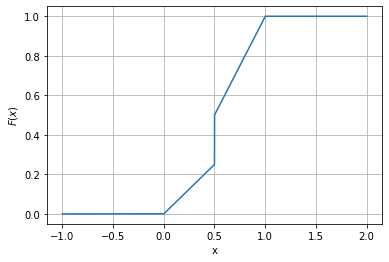
\includegraphics[width=\columnwidth]{solutions/ma/2015/27/Figure/fig4.png}
\caption{CDF of X}
\label{ma2015-27:fig:cdf}
\end{figure}

   

